\chapter{Testing} 

\begin{citazione}
Nell'ambito del presente capitolo verranno descritti i risultati ottenuti dalla fase di testing dell'algoritmo implementato. In primo luogo verrà descritto il \emph{Dataset} impiegato per il testing. Successivamente sarà presentato l'ambiente di esecuzione sul quale è stato eseguito l'algoritmo. In seguito verranno presentati i tempi di esecuzione di compressione e decompressione con i relativi rapporti di compressione effettuando un confronto tra i risultati ottenuti impiegando diversi algoritmi di \emph{variable length Prefix Code}. Infine verrà svolto un paragone tra i risultati ottenuti con la \emph{pipeline} proposta e quelli ottenuti mediante un compressore allo stato dell'arte.
\end{citazione}
\newpage

\section{Dataset}
Dal momento che l'algoritmo implementato lavora solo su testo, il \emph{Dataset} impiegato è costituito da diversi file di testo, di tipologia (racconti, codice sorgente, \dots) e lunghezza variabile. I suddetti file sono reperibili al seguente link: https://github.com/vincenzo-emanuele/Secure-Compression-based-on-BWT/tree/main/src/TestFiles/Input. 
\section{Ambiente di esecuzione}
Per svolgere la fase di testing dell'algoritmo implementato è stato utilizzato un \emph{MacBook Pro M1 (2020)} avente le seguenti specifiche:
\begin{itemize}
    \item S.O.: MacOS Montrey 12.2.1;
    \item CPU: Chip Apple M1;
    \item RAM: 8 GB;
    \item SSD : 512 GB;
    \item Versione di Python installata: 3.8;
\end{itemize}
\section{Risultati}\label{section:risultati}
La fase di testing condotta ha come scopo quello di verificare la bontà dell'algoritmo in termini computazionali (spazio e tempo) e di appurare che la decompressione vada a buon fine senza perdita di informazione, garantendo, dunque, che l'algoritmo di compressione implementato sia \emph{lossless}. Le tabelle \ref{tab:huffman}, \ref{tab:lzw}, \ref{tab:ac} e \ref{tab:bz2pipeline} indicano, per ogni file del \emph{Dataset}, la sua dimensione non compressa, la sua dimensione a seguito della compressione, il tempo impiegato per la compressione (corrisponde al tempo di esecuzione dello script \emph{compression.py} che implementa la \emph{pipeline} di compressione), il tempo impiegato per la decompressione (corrisponde al tempo di esecuzione dello script \emph{decompression.py} che implementa la \emph{pipeline} di decompressione) e il rapporto di compressione ottenuto. In particolare la prima tabella si riferisce alla \emph{pipeline} di compressione che utilizza \emph{Huffman} come algoritmo di \emph{variable length Prefix Code}, la seconda si riferisce alla \emph{pipeline} che fa uso di \emph{Lempel-Ziv-Welch}, la terza si riferisce alla \emph{pipeline} che fa uso di \emph{Arithmetic Coding} mentre la quarta si riferisce alla \emph{pipeline} che utilizza \emph{bzip2} nel suo passo finale.\\ La \emph{pipeline} di testing è implementata dallo script \emph{testing.py} a cui vanno passati i parametri da linea di comando che indicano il nome del file di input e la chiave segreta da utilizzare.\\
Come evidenziato dagli istogrammi \ref{fig:ist1}, \ref{fig:ist2} e \ref{fig:ist3}, non sono state riscontrate differenze evidenti tra l'utilizzo di \emph{Huffman} e quello di \emph{LZW}. Tendenzialmente \emph{Huffman} presenta tempi di esecuzione ed un rapporto di compressione leggermente migliori. Per quanto riguarda \emph{Arithmetic Coding}, è stato rilevato un lieve miglioramento in termini di rapporto di compressione a discapito di un tempo di esecuzione nettamente peggiore. La \emph{pipeline} che indubbiamente si comporta meglio è quella che utilizza \emph{bzip2} raggiungendo un rapporto di compressione più elevato rispetto a quello ottenuto con i precedenti algoritmi.
Dopo aver eseguito le fasi di compressione e decompressione, la \emph{pipeline} di testing si assicura che il processo sia avvenuto in maniera \emph{lossless}. Per fare ciò confronta il file di input con l'output della decompressione: se il contenuto di questi due differisce anche solo di un bit, comunicherà a video il fallimento della decompressione. Tale verifica ha restituito esito positivo su ognuno dei file del \emph{Dataset} utilizzato. Al fine di comprendere la bontà dell'algoritmo implementato è stata svolta un'attività di confronto con lo stato dell'arte della compressione mediante algoritmi basati sulla trasformata di \emph{Burrows-Wheeler}. In particolare il \emph{Dataset} utilizzato per testare l'algoritmo è stato sottoposto al compressore \textbf{bzip2} di cui è stata impiegata un'implementazione \emph{built-in} in \emph{Python} mediante la libreria \emph{bz2}. Dai confronti effettuati (di cui è disponibile un \emph{report} nella tabella \ref{tab:bzip2}) è emerso che \emph{bzip2} nella sua versione \emph{standalone} presenta un fattore di compressione leggermente migliore rispetto a quello della \emph{pipeline} proposta ed un tempo di esecuzione decisamente più basso sia in fase di compressione che in fase di decompressione.
%Huffman
%\begin{center}
    \begin{table}
    \begin{tabular}{||c c c c c c||} 
     \hline
     Input & Size non compr. & Size compr. & Tempo compr. & Tempo decompr. & \% \\ [0.5ex] 
     \hline\hline
     alice29.txt & 152.062 byte & 77.081 byte & 5.44 s & 0.41 s & 49.31\\ [1ex]
     \hline
     asyoulik.txt & 125.179 byte & 68.812 byte & 4.13 s & 0.36 s & 44.14\\ [1ex] 
     \hline
     cp.html & 24.603 byte & 12.342 byte & 0.15 s & 0.03 s & 49.83\\ [1ex] 
     \hline
     fields.c & 11.150 byte & 5.457 byte & 0.16 s & 0.03 s & 51.06\\ [1ex]
     \hline
     grammar.lsp & 3.721 byte & 2.295 byte & 0.04 s & 0.013 s & 38.33\\ [1ex] 
     \hline
     huffman.c & 6.986 byte & 3.582 byte & 0.04 s & 0.008 s & 48.73\\ [1ex]
     \hline
     lcet10.txt & 419.235 byte & 202.267 byte & 9.51 s & 0.70 s & 51.75\\ [1ex] 
     \hline
     manual.ps & 1.766.625 byte & 316.505 byte & 15.69 s & 1.58 s & 82.08\\ 
 [1ex]
     \hline
     plrabn12.txt & 481.861 byte & 265.393 byte & 10.07 s & 0.78 s & 44.92\\ [1ex] 
     \hline
     shrek.txt & 70.658 byte & 40.572 byte & 0.87 s & 0.09 s & 42.58\\ [1ex]

     \hline
    \end{tabular} 
    \caption{Risultati ottenuti con Huffman\label{tab:huffman}}
    \end{table}
%LZW
\begin{table}
    \begin{tabular}{||c c c c c c||} 
     \hline
     Input & Size non compr. & Size compr. & Tempo compr. & Tempo decompr. & \% \\ [0.5ex] 
     \hline\hline
     alice29.txt & 152.062 byte & 81.130 byte & 5.61 s & 0.26 s & 46.65\\ [1ex]
     \hline
     asyoulik.txt & 125.179 byte & 73.462 byte & 4.10 s & 0.22 s & 41.31\\ [1ex] 
     \hline
     cp.html & 24.603 byte & 13.832 byte & 0.40 s & 0.04 s & 43.78\\ [1ex] 
     \hline
     fields.c & 11.150 byte & 5.788 byte & 0.16 s & 0.02 s & 48.09\\ [1ex]
     \hline
     grammar.lsp & 3.721 byte & 2.347 byte & 0.04 s & 0.007 s & 36.93\\ [1ex] 
     \hline
     huffman.c & 6.986 byte & 3.813 byte & 0.09 s & 0.01 s & 45.42\\ [1ex]
     \hline
     lcet10.txt & 419.235 byte & 212.831 byte & 14.40 s & 1.004 s & 49.23\\ [1ex] 
     \hline
     manual.ps & 1.766.625 byte & 330.373 byte & 22.26 s & 2.58 s & 81.30\\ 
 [1ex]
     \hline
     plrabn12.txt & 481.861 byte & 281.687 byte & 15.04 s & 1.14 s & 41.54\\ [1ex] 
     \hline
     shrek.txt & 70.658 byte & 43.728 byte & 2.02 s & 0.13 s & 38.11\\ [1ex]

     \hline
    \end{tabular} 
    \caption{Risultati ottenuti con LZW\label{tab:lzw}}
    \end{table}
%\end{center} 

%Arithmetic Coding
%\begin{center}
    \begin{table}
    \begin{tabular}{||c c c c c c||} 
     \hline
     Input & Size non compr. & Size compr. & Tempo compr. & Tempo decompr. & \% \\ [0.5ex] 
     \hline\hline
     alice29.txt & 152.062 byte & 75.684 byte & 10.3 s & 13.58 s & 50.23\\ [1ex]
     \hline
     asyoulik.txt & 125.179 byte & 68.021 byte & 8.56 s & 12.19 s & 45.66\\ [1ex] 
     \hline
     cp.html & 24.603 byte & 12.792 byte & 0.94 s & 2.14 s & 48.01\\ [1ex] 
     \hline
     fields.c & 11.150 byte & 6.058 byte & 0.51 s & 1.01 s & 45.67\\ [1ex]
     \hline
     grammar.lsp & 3.721 byte & 2.996 byte & 0.21 s & 0.373 s & 19.48\\ [1ex] 
     \hline
     huffman.c & 6.986 byte & 4.217 byte & 0.26 s & 0.578 s & 39.64\\ [1ex]
     \hline
     lcet10.txt & 419.235 byte & 198.395 byte & 22.70 s & 36.29 s & 52.68\\ [1ex] 
     \hline
     manual.ps & 1.766.625 byte & 315.040 byte & 36.06 s & 59.14 s & 82.17\\ 
 [1ex]
     \hline
     plrabn12.txt & 481.861 byte & 260.351 byte & 27.11 s & 46.73 s & 45.97\\ [1ex] 
     \hline
     shrek.txt & 70.658 byte & 40.461 byte & 3.48 s & 7.15 s & 42.74\\ [1ex]

     \hline
    \end{tabular} 
    \caption{Risultati ottenuti con Arithmetic Coding\label{tab:ac}}
    \end{table}

%Bzip2-pipeline
%\begin{center}
    \begin{table}
    \begin{tabular}{||c c c c c c||} 
     \hline
     Input & Size non compr. & Size compr. & Tempo compr. & Tempo decompr. & \% \\ [0.5ex] 
     \hline\hline
     alice29.txt & 152.062 byte & 54.637 byte & 5.48 s & 0.38 s & 64.07\\ [1ex]
     \hline
     asyoulik.txt & 125.179 byte & 49.910 byte & 4.16 s & 0.39 s & 60.13\\ [1ex] 
     \hline
     cp.html & 24.603 byte & 9.568 byte & 0.16 s & 0.03 s & 61.11\\ [1ex] 
     \hline
     fields.c & 11.150 byte & 3.989 byte & 0.17 s & 0.04 s & 64.22\\ [1ex]
     \hline
     grammar.lsp & 3.721 byte & 1.684 byte & 0.05 s & 0.02 s & 54.74\\ [1ex] 
     \hline
     huffman.c & 6.986 byte & 2.721 byte & 0.05 s & 0.018 s & 61.05\\ [1ex]
     \hline
     lcet10.txt & 419.235 byte & 144.068 byte & 9.60 s & 0.78 s & 65.64\\ [1ex] 
     \hline
     manual.ps & 1.766.625 byte & 222.055 byte & 15.71 s & 1.76 s & 87.43\\ 
 [1ex]
     \hline
     plrabn12.txt & 481.861 byte & 188.980 byte & 10.19 s & 0.89 s & 60.79\\ [1ex] 
     \hline
     shrek.txt & 70.658 byte & 29.835 byte & 0.89 s & 0.11 s & 57.78\\ [1ex]

     \hline
    \end{tabular} 
    \caption{Risultati ottenuti con bzip2 nella pipeline\label{tab:bz2pipeline}}
    \end{table}

%BZIP2
\begin{table}
    \begin{tabular}{||c c c c c c||} 
     \hline
     Input & Size non compr. & Size compr. & Tempo compr. & Tempo decompr. & \% \\ [0.5ex] 
     \hline\hline
     alice29.txt & 152.062 byte & 43.172 byte & 0.016 s & 0.005 s & 71.61\\ [1ex]
     \hline
     asyoulik.txt & 125.179 byte & 39.569 byte & 0.013 s & 0.004 s & 68.39\\ [1ex] 
     \hline
     cp.html & 24.603 byte & 7.624 byte & 0.003 s & 0.0007 s & 69.01\\ [1ex] 
     \hline
     fields.c & 11.150 byte & 3.039 byte & 0.002 s & 0.0003 s & 72.74\\ [1ex]
     \hline
     grammar.lsp & 3.721 byte & 1.283 byte & 0.0009 s & 0.0002 s & 65.52\\ [1ex] 
     \hline
     huffman.c & 6.986 byte & 2.110 byte & 0.001 s & 0.0003 s & 69.80\\ [1ex]
     \hline
     lcet10.txt & 419.235 byte & 107.648 byte & 0.03 s & 0.009 s & 74.32\\ [1ex] 
     \hline
     manual.ps & 1.766.625 byte & 162.220 byte & 0.37 s & 0.03 s & 90.82\\ 
 [1ex]
     \hline
     plrabn12.txt & 481.861 byte & 145.545 byte & 0.04 s & 0.01 s & 69.80\\ [1ex] 
     \hline
     shrek.txt & 70.658 byte & 23.346 byte & 0.006 s & 0.003 s & 66.96\\ [1ex]

     \hline
    \end{tabular} 
    \caption{Risultati ottenuti con bzip2\label{tab:bzip2}}
    \end{table}
\begin{figure}[h]
    \centering
    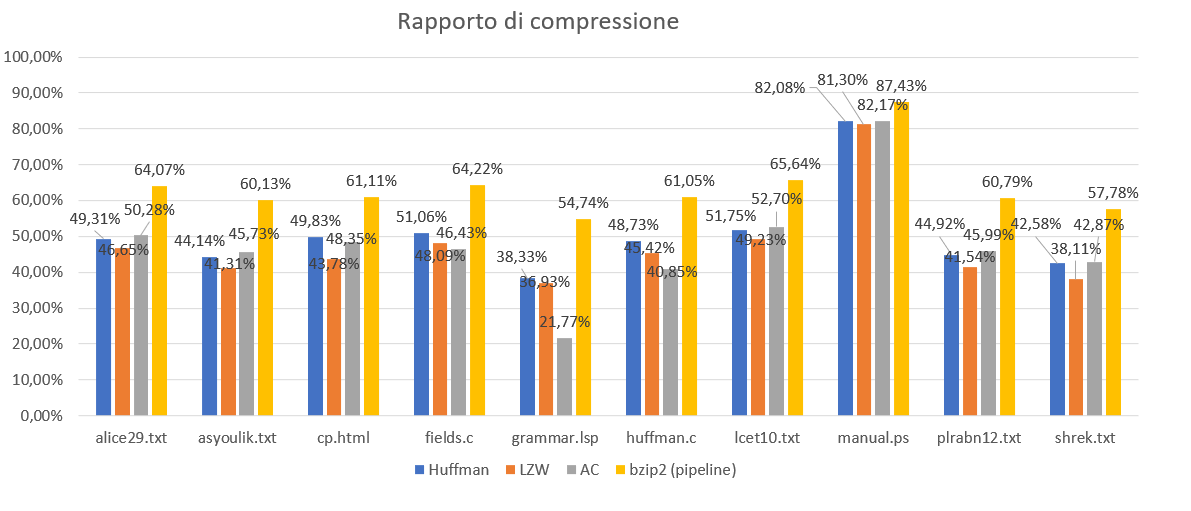
\includegraphics[scale=0.5]{Progetto Compressione Dati/capitoli/images/compression_rate.png}
\caption{Rapporto di compressione}
    \label{fig:ist1}
\end{figure} 
\begin{figure}[h]
    \centering
    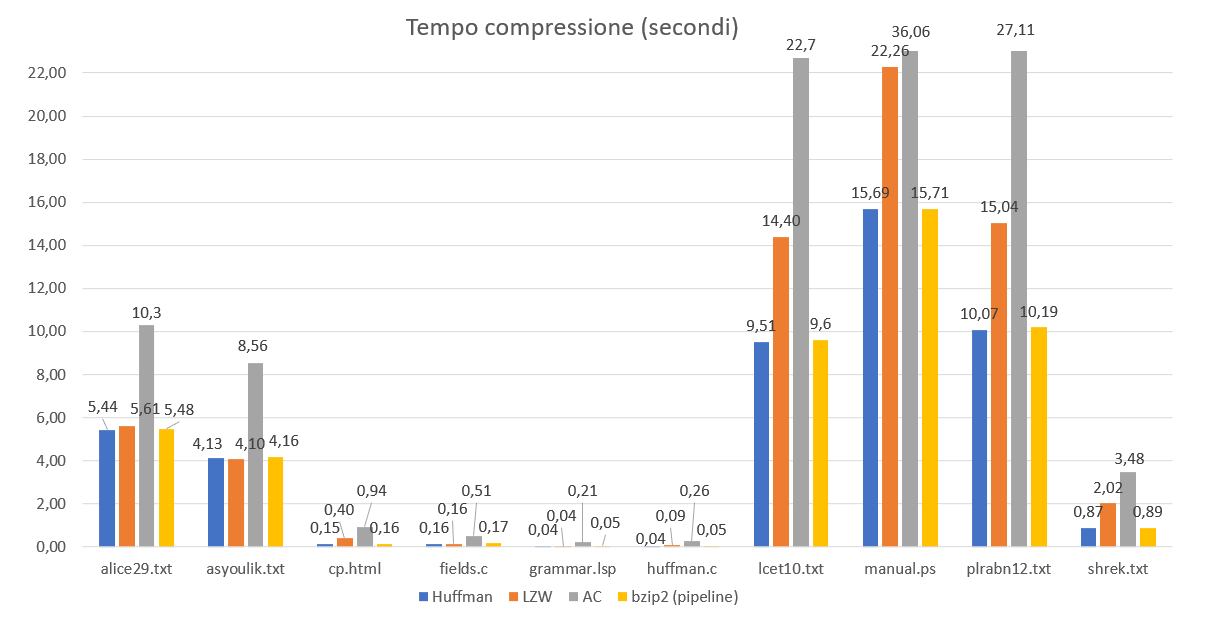
\includegraphics[scale=0.5]{Progetto Compressione Dati/capitoli/images/compression_time.png}
\caption{Tempo di compressione}
    \label{fig:ist2}
\end{figure} 
\begin{figure}[h]
    \centering
    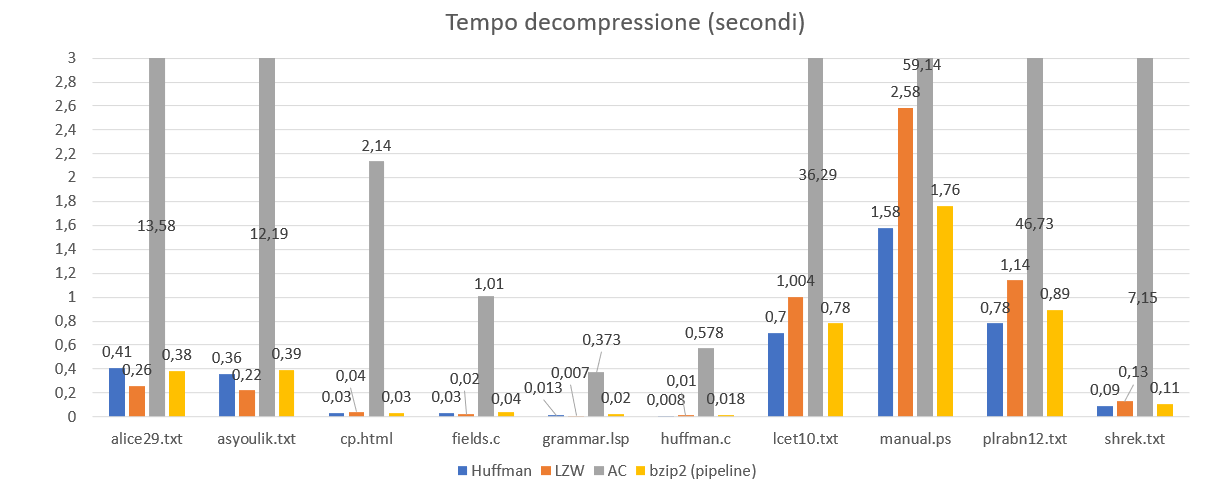
\includegraphics[scale=0.5]{Progetto Compressione Dati/capitoli/images/decompression_time.png}
\caption{Tempo di decompressione}
    \label{fig:ist3}
\end{figure} 